\section{CT invention: Electron-beam CT} %US 4352021 A (Boyd, 1982)
Our next assessment deals with an innovation related to computed tomography. In
particular, we take a closer look at Electron-beam Computed Tomography (EBCT),
also know as Ultrafast CT.

\subsection{Defining the technology}
Traditional CT scanners have an X-ray tube embedded in the toroid body. By
mechanically rotating the tube along with the detector, projections from an
arbitrary angle can be captured.

EBCT also needs to be able to capture projections from any angle, but takes
another route. Remember that in a regular X-ray tube current flowing through the
cathode releases electrons. The electrons are accelerated towards the anode by
applying a voltage across the tube. When the electrons hit the anode at high
speed, they release part of their energy as X-rays. The same principle is used
in EBCT, except that the tube is physically split up in two dedicated parts. One
is the cathode or electron gun and is placed along the patient's longitudinal
axis. The other is the anode and is shaped in a semi-ring around the patient.
Using magnetic fields, the electrons fired from the cathode are deflected onto this
ring, where they produce X-rays that can be captured by a detector array as
usual \cite{suetens}. \autoref{fig:ebctscanner} illustrates this.

\begin{figure}[ht]
\begin{center}
  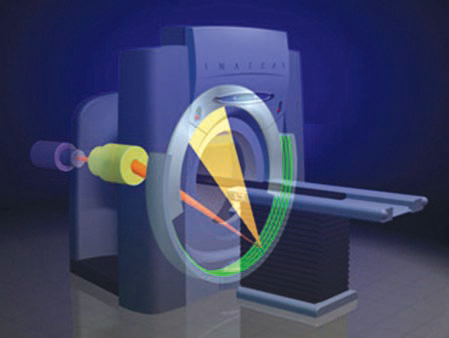
\includegraphics[width=\linewidth]{img/EBCT.png}
  \caption{Rendering of an EBCT scanner's inner workings \cite{suetens}.}
  \label{fig:ebctscanner}
\end{center}
\end{figure}

The main advantage of this setup is that the X-ray source rotation is no longer
mechanical. This allows for faster sweeps, which in turn make it easier to image
moving structures such as the heart. One very prominent application is the
detection of calcifications from atherosclerosis in the coronal arteries
\cite{ultrafastcad}. These are very close to the heart, and can move by about
five times their own diameter every heartbeat. 

More recently, these EBCT scanners have received strong competition from
multislice helical CT scanners. The latter enjoy a widespread adoption and are
also less costly. However, their rotation speed still cannot match that of
Ultrafast CT \cite{ultravshelical}. In addition, this techniques requires a
lower dose compared to traditional CT, and much lower than a CT angiography
\cite{ultralowdose}.

In conclusion, this technique is promising for non-invasive detection of
coronary heart disease, but it has too many unsolved problems to replace general
purpose CT scanners \cite{multictbook}.

\subsection{Assessing novelty in functionality}

\subsubsection{Novelty in components}
As outlined above, the components are largely the same as in conventional CT
scanners. Only their location is different. One additional component is the coil
to generate the deflecting magnetic field. Such electromagnets were used before
in imaging, particularly in MRI, but for a very different purpose.

\subsubsection{Novelty in natural effects exploited}
The same story applies for novelty in natural effects exploited: few new effects
except bending of the electron beam using magnetic fields. The same principle
was used much earlier in Cathode Ray Tube (CRT) monitors and televisions.

\subsubsection{Scores}
In \autoref{tbl:funcscores2} we give an overview of the scores on the various
topics.

\begin{table}[h]
\centering
\begin{tabular}{l l}
\hline
\multicolumn{2}{|c|}{Novelty in functionality} \\
\hline
A. Novelty of components & B. Novelty in natural effects exploited\\
A1) 3 & B1) 3\\ 
A2) 5 & B2) 5\\ 
\hline
\end{tabular}
\caption{Novelty in functionality scores}
\label{tbl:funcscores2}
\end{table}

\subsection{Assessing novelty in knowledge origins}
Again, we look into the problems that had to be solved to find the knowledge
origins. We only look at the problems that are different in comparison to a
traditional CT scanner.

Problem 1: deflect the electron beam onto the anode ring.

Solution 1: use magnetic fields (electric field deflection only works for small angles)

KO1: electromagnetism, CRT monitors

Problem 1.1: overcoming Coulomb repulsion to obtain proper beam focus

Solution 1.1: leak nitrogen into vacuum chamber \cite{ebctelectric}

KO 2: charged particle optics

Problem 2: synchronise imaging with heart rhythm

Solution 2: use ECG equipment

KO3: biomedical sensors, signal processing

\subsubsection{Scores}
Electromagnetism, charged particle optics and signal processing can be
considered scientific origins, while the others are technological in nature.

Note that using ECG equipment to synchronise imaging with the heart rhythm is
not new. It was occasionally used before in various other imaging modalities
\cite{suetens}.

\begin{table}[h]
\centering
\begin{tabular}{l l}
\hline
\multicolumn{2}{|c|}{Novelty in knowledge origins} \\
\hline
A. Novelty of scientific origins & B. Novelty of technological origins\\
A1) 4 & B1) 5\\ 
A2) 1 & B2) 1\\ 
\hline
\end{tabular}
\caption{Novelty in knowledge origins scores}
\label{tbl:origscores2}
\end{table}

\subsection{Assessing technological impact}
\subsubsection{Performance increase}
As outlined above, EBCT is very useful for mainly one thing: imaging the heart
and its periphery. However, there are serious drawbacks that do not make it
useful as a general purpose CT scanner. For example, due to the new geometry
X-ray scatter cannot be reduced as effectively. This in turn generates extra
artifacts on the resulting image. The electron gun also has limited power making
it inadequate for higher dosage (i.e., higher contrast) studies \cite{multictbook}.

\subsubsection{Technological accumulation}
\paragraph{Broadness of impact}

\paragraph{Magnitude of impact}

\paragraph{Novelty of impact}

\subsubsection{Obsoleting previous technologies}
EBCT has definitely not obsoleted previous technologies. Its area of use is
simply too limited for many hospitals to warrant such an expensive purchase.
Instead, older and cheaper but less effective methods are still used more often
to diagnose coronary artery disease. Examples include exercise stress tests but
also invasive (catheter) examinations.

\subsubsection{Scores}
\begin{table}[h]
\centering
\begin{tabular}{l l l}
\hline
\multicolumn{3}{|c|}{Technological impact} \\
\hline
A. Performance increase & B. Tech. accumulation & Obsoleting previous tech.\\
A) 5 & B1 a)  --- b)  & C) 2\\ 
     & B2 a)  --- b)  & \\
     & B3 a)  --- b)  & \\
\hline
\end{tabular}
\caption{Technological impact scores}
\label{tbl:impactscores2}
\end{table}